\section{Squark Production at One-Loop}


\subsection{The LSZ Theorem}\label{sec:LSZ}
The LSZ theorem\cite{Lehmann:1954rq} or LSZ reduction formula prescribes how to obtain the S-matrix element, i.e. a physical observable, from the time ordered correlation function of the respective field operators. The time ordered correlation function of fields in an interacting theory can be calculated perturbatively with the aid of the Gell-Mann and Low theorem and the Wick theorem. \\
Considering a physical process with kinematics $\vec{k}_1 \hdots \vec{k}_n \to \vec{p}_1 \hdots \vec{p}_m$ and taking for the sake of simplicity only one scalar field $\phi$ the Fourier transform of the time ordered product of a correlation function is related to the corresponding S-matrix element like\footnote{In this subsection the $\sim$ indicates that the poles on either side are the same provided that all momenta are close to their mass shell, i.e. $p_i^0 \to E_{\vec{p}_i}$ and $k_j^0 \to E_{\vec{k}_j}$.}
\begin{align}
\prod_{i=1}^n \int \mathrm{d}x_i\ \mathrm{e}^{ip_i x_i} \prod_{j=1}^m \int \mathrm{d}y_j\ \mathrm{e}^{ik_j y_j} \left\langle \Omega | \mathcal{T} \left[ \phi(x_1) \hdots \phi(x_n) \phi(y_1) \hdots \phi(y_m) \right] | \Omega\right\rangle \nonumber\\
\sim \prod_{i=1}^n \frac{i\sqrt{Z}}{p_i^2 - m^2 + i\epsilon} \prod_{j=1}^m \frac{i\sqrt{Z}}{k_j^2 - m^2 + i\epsilon} \left\langle \left.\left.\vec{p}_1 \hdots \vec{p}_n \right| S \right| \vec{k}_1 \hdots \vec{k}_m \right\rangle .\label{eq:LSZ}
\end{align}
Here $\mathcal{T}$ denotes the time ordering operator, $\left.| \Omega \right\rangle$ is the ground state of the interacting theory and $\sqrt{Z}$ is the residue of the single particle pole in the two-point function 
\begin{align}
\int \mathrm{d}x\ \mathrm{e}^{ip x} \left\langle \Omega | \mathcal{T} \left[ \phi(x) \phi(0) \right] | \Omega\right\rangle &= \frac{i}{p^2-m_0^2} + \frac{i}{p^2-m_0^2} \left(\frac{i\Sigma(p^2)}{p^2-m_0^2}\right) + \frac{i}{p^2-m_0^2} \left(\frac{\Sigma(p^2)}{p^2-m_0^2}\right)^2 + \hdots\nonumber\\
&= \frac{i}{p^2 - m_0^2 - \Sigma(p^2)}.\label{eq:propagator}
\end{align}
\begin{figure}[!htbp]
\begin{center}
\begin{tikzpicture}[line width=2.0 pt, scale=1.3]
	\draw[fermionnoarrow](180:1)--(180:0.5);	
	\draw (0,0) circle (.5cm);
		\begin{scope}
	    	\clip (0,0) circle (.5cm);
	    	\foreach \x in {-1.0,-0.9,...,1.0}
        \draw[line width=1 pt] (\x,-.5) -- (\x+.6,.5);
	  	\end{scope}
	\draw[fermionnoarrow](0:0.5)--(0:1);
	\node at (1.3,0) {=};
	\draw[fermionnoarrow](0:1.6)--(0:2.6);
	\node at (2.9,0) {+};
    \draw[fermionnoarrow](0:3.2)--(0:3.7);	
	\draw (4.2,0) circle (.5cm);
	\node at (4.2,0) {1PI};
	\draw[fermionnoarrow](0:4.7)--(0:5.2);
	\node at (5.5,0) {+};	
	\draw[fermionnoarrow](0:5.8)--(0:6.3);	
	\draw (6.8,0) circle (.5cm);
	\node at (6.8,0) {1PI};
	\draw[fermionnoarrow](0:7.3)--(0:7.8);
	\draw (8.3,0) circle (.5cm);
	\node at (8.3,0) {1PI};
	\draw[fermionnoarrow](0:8.8)--(0:9.3);
	\node at (9.8,0) {+ $\hdots$};
\end{tikzpicture}
\caption{Diagrammatic figure of the two-point function of a scalar field: The propagator in an interaction theory can be calculated in a perturbation series in the coupling constant.}\label{fig:fullpropagator}
\end{center}
\end{figure}
The parameter $m_0$ is the tree-level mass and the quantity $-i \Sigma(p^2)$ denotes the sum of all one-particle-irreducible contributions to the particle's self-energy. From eq. \ref{eq:propagator} one can read off the physical mass $m^2$ of the particle which is associated with the field $\phi$. It is determined as the value of $p^2$ where the propagator has a pole, i.e. 
\begin{align}
\left[ p^2 - m_0^2 - \Sigma(p^2)\right]_{p^2 = m^2} = 0
\end{align}
Close to the pole the denominator of eq. \ref{eq:propagator} can by expanded like
\begin{align}
p^2 - m_0^2 - \Sigma(p^2) = (p^2 - m^2)\left( 1 - \frac{\partial \Sigma(p^2)}{\partial p^2} \right)_{p^2 = m^2} + \mathcal{O}((p^2 - m^2)^2).
\end{align}
The residue of the propagator can therefore be written as 
\begin{align}
Z = \left( 1 - \frac{\partial \Sigma(p^2)}{\partial p^2} \right)_{p^2 = m^2}^{-1}.
\end{align}
Now considers the full $(n+m)$-point function in scalar theory. One can decompose it into an amputated $(n+m)$-point function and "full" propagators like written in eq. \ref{eq:propagator} and depicted in fig. \ref{fig:fullpropagator}.
\begin{figure}[!htbp]
\begin{center}
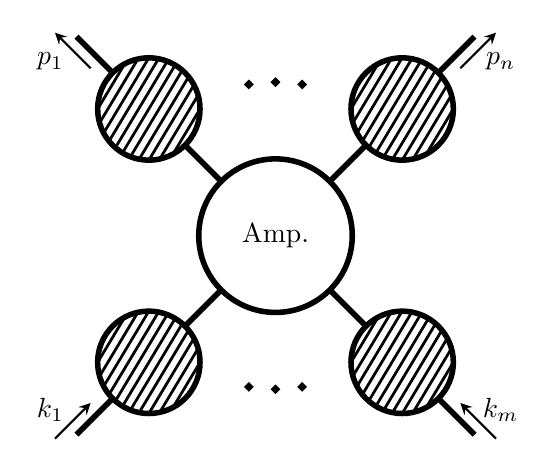
\begin{tikzpicture}[line width=2.0 pt, scale=1.3, arrow/.style={thick,->,shorten >=2pt,shorten <=2pt,>=stealth}]
	\draw (0,0) circle (.75);
	\node at (0,0) {Amp.};
	\draw (45:0.75)--(45:1.25);
	\draw (45:1.75) circle (.5);
		\begin{scope}[shift={(45:1.75)}]
	    	\clip (0,0) circle (.5cm);
	    	\foreach \x in {-1.0,-0.9,...,1.0}
        \draw[line width=1 pt] (\x,-.5) -- (\x+.6,.5);
	  	\end{scope}
	\draw (45:2.25)--(45:2.75);
	\draw[arrow] (1.768,1.597)--(2.192,2.021);
	\node at (2.2,1.7){$p_n$};

	\draw (135:0.75)--(135:1.25);
	\draw (135:1.75) circle (.5);
		\begin{scope}[shift={(135:1.75)}]
	    	\clip (0,0) circle (.5cm);
	    	\foreach \x in {-1.0,-0.9,...,1.0}
        \draw[line width=1 pt] (\x,-.5) -- (\x+.6,.5);
	  	\end{scope}
	\draw (135:2.25)--(135:2.75);
	\draw[arrow] (-1.768,1.597)--(-2.192,2.021);
	\node at (-2.2,1.7){$p_1$};	
	
	\draw (225:0.75)--(225:1.25);
	\draw (225:1.75) circle (.5);
		\begin{scope}[shift={(225:1.75)}]
	    	\clip (0,0) circle (.5cm);
	    	\foreach \x in {-1.0,-0.9,...,1.0}
        \draw[line width=1 pt] (\x,-.5) -- (\x+.6,.5);
	  	\end{scope}
	\draw (225:2.25)--(225:2.75);
	\draw[arrow] (-2.192,-2.021)--(-1.768,-1.597);
	\node at (-2.2,-1.7){$k_1$};	
	
	\draw (315:0.75)--(315:1.25);
	\draw (315:1.75) circle (.5);
		\begin{scope}[shift={(315:1.75)}]
	    	\clip (0,0) circle (.5cm);
	    	\foreach \x in {-1.0,-0.9,...,1.0}
        \draw[line width=1 pt] (\x,-.5) -- (\x+.6,.5);
	  	\end{scope}
	\draw (315:2.25)--(315:2.75);
	\draw[arrow] (2.192,-2.021)--(1.768,-1.597);
	\node at (2.2,-1.7){$k_m$};
	
	\draw[fill=black] (80:1.5) circle (.01);
	\draw[fill=black] (90:1.5) circle (.01);
	\draw[fill=black] (100:1.5) circle (.01);
	\draw[fill=black] (-80:1.5) circle (.01);
	\draw[fill=black] (-90:1.5) circle (.01);
	\draw[fill=black] (-100:1.5) circle (.01);
\end{tikzpicture}
\caption{Diagrammatic figure of a "full" $(n+m)$-point function. Apart from the "full" propagators there is the "full" amputated $(n+m)$-point function}
\end{center}
\end{figure}\\
Inserting the expression
\begin{align}
\frac{i}{p^2 - m_0^2 - \Sigma(p^2)} \sim \frac{i Z}{p^2 - m^2}
\end{align}
for the full propagators one notices the same singularity as in eq. \ref{eq:LSZ}. If one now compares the coefficients of these poles in eq. \ref{eq:LSZ} one finds
\begin{figure}[!htbp]
\begin{center}
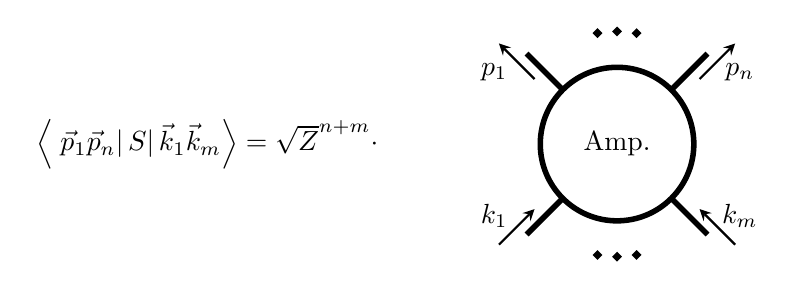
\begin{tikzpicture}[line width=2.0 pt, scale=1.3, arrow/.style={thick,->,shorten >=2pt,shorten <=2pt,>=stealth}]
	\node at (-4,0) {$\left\langle \left.\left.\vec{p}_1 \hdots \vec{p}_n \right| S \right| \vec{k}_1 \hdots \vec{k}_m \right\rangle =\sqrt{Z}^{n+m} \cdot$};
	\draw (0,0) circle (.75);
	\node at (0,0) {Amp.};

	\draw (45:0.75)--(45:1.25);
	\draw[arrow] (0.768,0.597)--(1.192,1.021);
	\node at (1.2,0.7){$p_n$};

	\draw (135:0.75)--(135:1.25);
	\draw[arrow] (-0.768,0.597)--(-1.192,1.021);
	\node at (-1.2,0.7){$p_1$};	
	
	\draw (225:0.75)--(225:1.25);
	\draw[arrow] (-1.192,-1.021)--(-0.768,-0.597);
	\node at (-1.2,-0.7){$k_1$};	
	
	\draw (315:0.75)--(315:1.25);
	\draw[arrow] (1.192,-1.021)--(0.768,-0.597);
	\node at (1.2,-0.7){$k_m$};
	
	\draw[fill=black] (80:1.1) circle (.01);
	\draw[fill=black] (90:1.1) circle (.01);
	\draw[fill=black] (100:1.1) circle (.01);
	\draw[fill=black] (-80:1.1) circle (.01);
	\draw[fill=black] (-90:1.1) circle (.01);
	\draw[fill=black] (-100:1.1) circle (.01);
\end{tikzpicture}
\end{center}
\end{figure}\\
Now it becomes visible why the renormalization in the on-shell scheme
\begin{align}
\left.\frac{\partial \Sigma(p^2)}{\partial p^2}\right|_{p^2 = m^2} \stackrel{!}{=} 0
\end{align}
introduces no further manipulation when turning from the correlation function to the S-matrix-element because $Z = 1$ in on-shell renormalization. Furthermore the on-shell condition for the mass renormalization
\begin{align}
\Sigma(p^2)|_{p^2 = m^2} = 0
\end{align}
means that the physical mass equals the tree level mass.

\subsection{The Squark Production Cross Section at Next-to-Leading Order}
\begin{figure}[!htpb]
\begin{center}
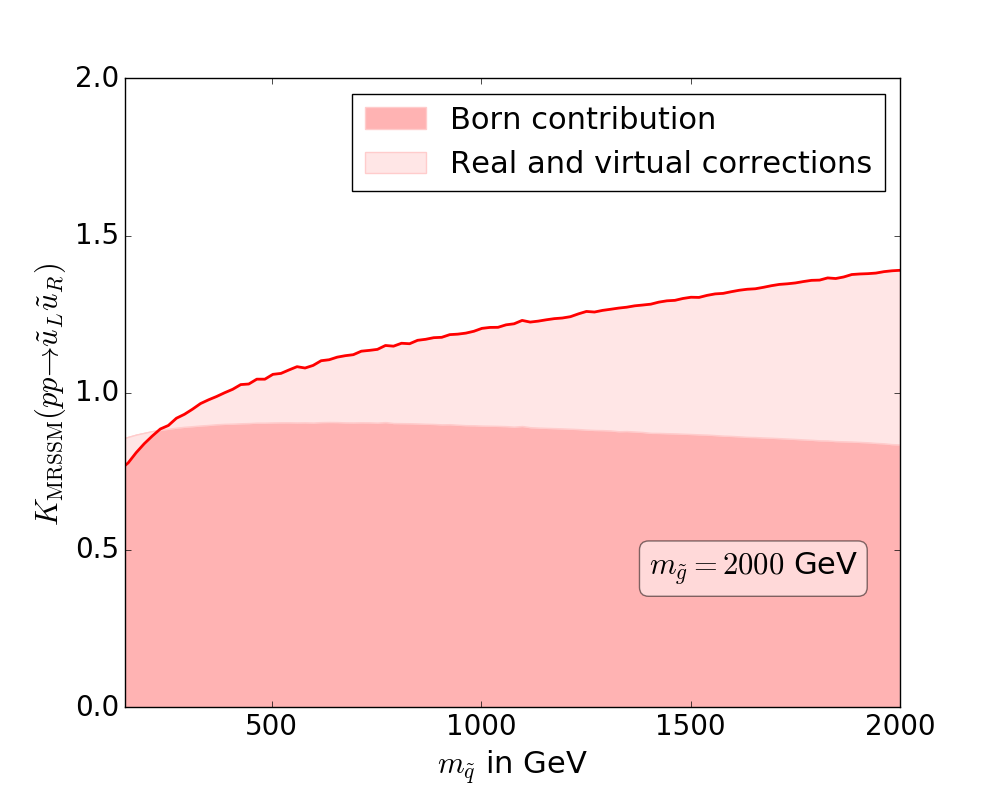
\includegraphics[scale=.5]{figures/MRSSM_uu_susu_Kfactors_msg=2000GeV.png}
\caption{}\label{fig:1LXsection_fixed_m}
\end{center}
\end{figure}
Calculate uncertainties for one point(pdf, scale, integration)


\subsection{The Cross Section in the Limit of Large Sgluon Masses}
The cross section for squark production does not exist in the limit of an infinitely large sgluon mass, instead it was found that it diverges logarithmically.\\
\begin{align}
\lim_{m_{\sigma^0}\to\infty} \sigma(qq \to \tilde{q}\tilde{q}) \sim \ln \frac{m_{\sigma^0}^2}{\mu^2}
\end{align}
This is actually expected as an effective field theory of the MRSSM where the sgluon is integrated out is no longer supersymmetric. This is because the sgluon is together with the octino part of a supermultiplet. Integrating out only the sgluon means that the octino misses its superpartner in the effective field theory. In this case the decoupling theorem \cite{Appelquist:1974tg} does no longer hold.\\
Refer to super oblique correction and quantify difference of $g$ and $\hat{g}$ from eq 4 in \cite{Cheng:1997sq}\\
append plot